\documentclass[10pt,a4paper]{report}
\usepackage[utf8]{inputenc}
\usepackage[german]{babel}
\usepackage[T1]{fontenc}
\usepackage{amsmath}
\usepackage{amsfonts}
\usepackage{amssymb}
\usepackage{graphicx}
\author{Julian Sobott (76011), David Sugar (76050), Lukas Mendel (76009)}
\title{Bericht Datenbank Praktikum}
\begin{document}
\maketitle
\tableofcontents

\newpage
\section{Aufgabe 1}
\subsection{a)}
\begin{figure}[h]
	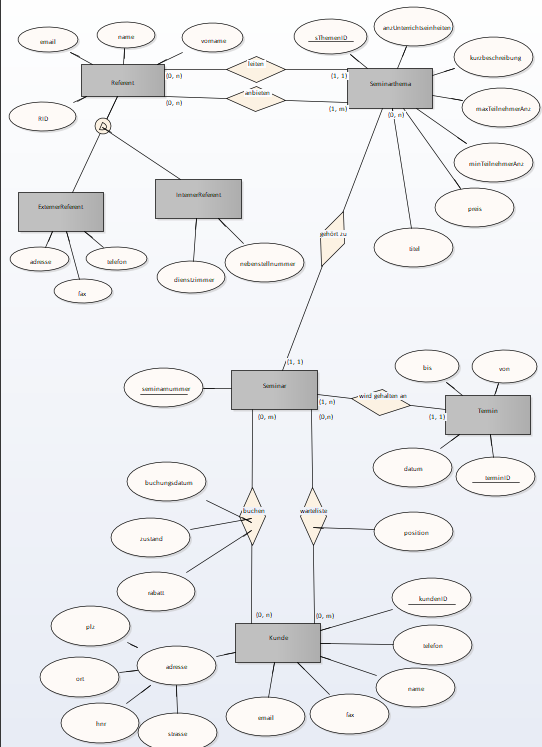
\includegraphics[scale=0.7]{Bilder/ER-Modell.PNG}
	\caption{ER-Modell Seminarverwaltung}
	\label{er:1}
\end{figure}

\subsubsection{Entities}
seminar = (\{\underline{SEMINARNUMMER:VARCHAR}\})

termin  = (\{\underline{TERMINID:VARCHAR}, DATUM:DATE, VON:DATETIME, BIS:DATETIME\})

kunde   = (\{\underline{KUNDENID:VARCHAR}\})

referent = (\{RID: Integer, email: VARCHAR, name: VARCHAR, vorname: VARCHAR\})

seminarthema = (sThemaID: Integer, anzUnterrichtseinheiten: Integer, kurzbeschreibung:VARCHAR, maxTeilnehmerAnz: Integer, minTeilnehmerAnzahl: Integer, preis: Float, titel: VARCHAR\})

externerReferent = (\{adresse: (plz: VARCHAR, ort: VARCHAR, strasse: VARCHAR, hnr: VARCHAR)\})

internerReferent = (\{dienstzimmer: VARCHAR, nebenstellnummer: Integer\})

\subsubsection{Relations}

leiten = (referent X seminarthema)

anbieten = (referent X seminarthema)

is\_a = (referent X sxternerReferent)

is\_a = (referent X internerReferent)

gehört\_zu = (seminarthema X seminar)

buchen = (seminar x kunke, BUCHUNGSDATUM:DATE, ZUSTAND:VARCHAR, RABATT:FLOAT)

warteliste = (kunde x seminar, POSITION:INTEGER)

wird\_gehalten\_an = (seminar x termin)



\subsection{b)}

\end{document}
